% JuliaCon proceedings template
\documentclass{juliacon}
\usepackage{xspace}
\setcounter{page}{1}

\begin{document}

\newcommand{\chipsort}{{\tt ChipSort}\xspace}

% **************GENERATED FILE, DO NOT EDIT**************

\title{ChipSort: a SIMD and cache-aware sorting module}

\author[]{Nicolau Leal Werneck}
\affil[]{TomTom NV}

\keywords{Julia, Sorting, SIMD, Parallelism, Metaprogramming}



\maketitle

\begin{abstract}

Sorting is a fundamental programming problem with many important applications. While there are well-known sorting algorithms for conventional computers, especial techniques are required to take the most out of real hardware offering features such as cache memory and instruction-level parallelism. ChipSort is a Julia module for SIMD and cache-aware sorting. It implements sorting networks and bitonic merge networks with SIMD instructions, with configurable vector sizes. It also implements Combsort, which lends itself easily to vectorization and can achieve good performance depending on the memory access cost. Insertion sort is used to finalize. Large arrays are approached with a multi-way Mergesort. The implementation of ChipSort itself is of interest from a programming languages perspective due to its use of metaprogramming, and more specifically Julia's generated functions. This permits tuning the code to specific tasks and hardware at runtime, a feat owed to Julia. This article presents the implemented techniques as well as experiments that demonstrate speed gains compared to multiple standard libraries.

\end{abstract}

\section{Introduction}

Sorting has enjoyed an important place within computer programming topics for a long time. Apart from having great importance in practical applications, being very useful to organize data for fast retrieval, it also attracts attention as a theoretically interesting problem in itself~\cite{DBLP:books/lib/Knuth98a}. While sorting is a well-understood problem in general, with a few classic algorithms available, achieving optimal performance for specific problems and architectures may require a careful algorithm selection rather than just tuning parameters \cite[Part II, Introduction]{DBLP:books/daglib/0023376}.

The running time of a computer program is governed by many factors, starting with algorithmic complexity and the base clock speed of the processor. The performance observed in real computers has been increasingly depending in processor features that are not taken into account by the simplest models, though. These features include cache memory and paralellism at the processor and instruction levels. Cache memory has become popular in consumer processors in the past couple of decades, allowing programs to often attain higher performance than would be possible with a simpler memory architecture, as long as memory access patterns exhibit temporal and spatial locality~\cite[Chapter 3]{Drepper07whatevery}. Writing software that can better cope with parallelism has also become necessary to exploit the full potential offered by modern and future processors~\cite{wilson2018}.

The interest in sorting and the great relevance of cache memory and parallelism in modern computing naturally led to research on sorting algorithms that account for these factors. Processors offering SIMD (single instruction, multiple data) instructions and other forms of instruction-level parallelism started to become widely available in the early 2000s. One example is the introduction of SSE instructions in the x86 architecture~\cite[Chapter 1]{kusswurm18}. The current availability of processors with 512 bit registers underscores the need of being able to write software that exploits vector operations, not to mention GPUs.

At the time SIMD CPUs became widely available there was already a trend to employ specialized hardware like GPUs for scientific applications~\cite{larsen2001fast,DBLP:conf/micro/ThompsonHO02}. Although SIMD was used mostly for multimedia applications at first~\cite{CHEN2006509,DBLP:journals/mam/SlingerlandS05}, some early alternative uses include 3D graphics~\cite{DBLP:conf/pcm/MaY02} and machine learning~\cite{DBLP:conf/europar/StreyB01}.

Following earlier work on parallel sorting in other architectures, the late 2000s saw the first practical demonstrations of sorting with modern consumer SIMD chips~\cite{DBLP:conf/IEEEpact/InoueMKN07,DBLP:journals/pvldb/ChhuganiNLMHCBKD08}. Most of the techniques utilized then are still employed in more recent works~\cite{DBLP:journals/pvldb/BalkesenATO13,DBLP:journals/pvldb/InoueT15}.

This article presents \chipsort, a Julia module that implements SIMD and cache-aware sorting utilizing some of the techniques found in the literature. These include sorting and merging networks, the use of Combsort for medium sized arrays and of multi-way merging for large arrays. These techniques require not only tuning parameters such as vector and array sizes, but also generating specific code when implementing different size networks. \chipsort seeks to generate efficient custom code for each task, relying on Julia metaprogramming capabilities for that.

Section~\ref{sec:methods} ahead presents the techniques employed in \chipsort. Section~\ref{sec:experiments} presents experimental results assessing the performance of the module and Section~\ref{sec:conclusion} brings some concluding remarks.

\section{SIMD sorting techniques}
\label{sec:methods}
%
\chipsort offers four high-level functions that can be used in applications as replacements for other sorting functions such as \verb sort  in the Julia standard library. Additional work may be required from the user selecting among the functions and also setting some numeric parameters. The {\tt chipsort!} function does not require any configuration and offers a great performance in a wide range of cases. The remaining functions are intended to be used with arrays of different sizes, and \verb chipsort_large  offers a good overview of all the techniques implemented in the module. Some of these techniques might also be useful in other applications instead of sorting, one clear example being the in-place matrix transpose. \chipsort does not currently support data records with separate key and payload, what might allow significant optimizations. Only the sorting of simple data types such as 32 and 64-bit integers and floating-point numbers has been studied so far.

This section will present how \verb chipsort_large  works, detailing each step of the process. It mostly follows~\cite{DBLP:journals/pvldb/InoueT15} with a few modifications. This function achieves sorting by first splitting the input array in chunks that are sorted separately with \verb chipsort_medium!  and then merged simultaneously. This inner sort is performed in multiple steps:
\begin{enumerate}
\item sorting small blocks of data with a sorting network;
\item reordering vectors in-place according to a matrix transpose;
\item vectorized Combsort with a limited number of iterations;
\item regular insertion sort until the whole data is sorted.
\end{enumerate}

The remainder of this section will detail the multiple techniques employed in this process.

\subsection{Sorting networks}
%
Sorting networks~\cite[Sec. 5.3.4]{DBLP:books/lib/Knuth98a} are graphs composed by comparator modules, units that take two numbers in, and output them in order: the smallest and the largest at specific outputs. Properly arranging the compatators allows the creation of a procedure that takes a vector of numbers in, and outputs them in sequence. The design of a sorting network can minimize the total number of comparisons, or also take into account that comparisons can be done in parallel, minimizing the number of steps to complete the process.

A sorting network can be represented by a Knuth graph such as Figure~\ref{fig:sorting-network}. The graph represents a network that takes an array of four values $(A_1, A_2, A_3, A_4)$ and outputs the sorted sequence $(S_1, S_2, S_3, S_4)$. Each vertical line in the graph represents a comparator.
\begin{figure}[htb]
\centerline{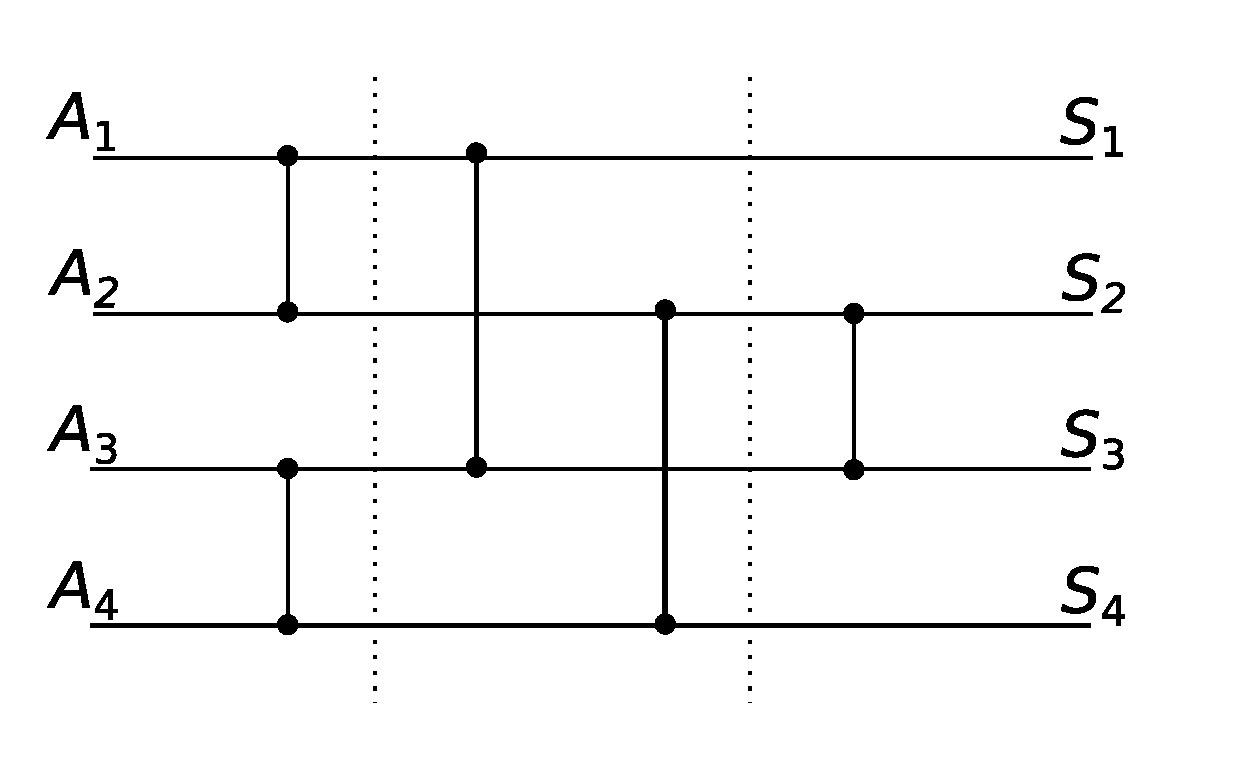
\includegraphics[width=0.6\linewidth]{fig/sorting-network-4.pdf}}
\caption{A sorting network for 4 elements. The dashed lines delimit each step where operations are independent of each other.}
\label{fig:sorting-network}
\end{figure}

In \chipsort, as in the related work, parallelism is mainly exploited by carrying out the comparisons of the sorting network over vectors of size $V$ contained in SIMD registers, effectively running the network $V$ times simultaneously. Other forms of instruction-level parallelism can also be in play, though. In especial, it may also be possible to parallelize instructions such as \verb min  and \verb max , and also the loading of data into registers. This is often done implicitly by the microarchitecture, and programmers can only try to make sure their code is suitable for this by properly ordering operations and avoiding branching, for instance. Part of this work is expected to be performed by the compiler, and especially LLVM in the case of Julia.

\chipsort supports sorting networks of different sizes, currently only powers of 2, which are predefined as data structures in the file \href{https://github.com/nlw0/\chipsort.jl/blob/d2d049b7413f0073476021fa62fb748803130768/src/sorting-network-parameters.jl}{\tt sorting-network-parameters.jl}. The generated function \href{https://github.com/nlw0/\chipsort.jl/blob/d2d049b7413f0073476021fa62fb748803130768/src/sorting-networks.jl#L13}{\tt sort\_net} works by assigning each element of the sequence at each step to a variable, and calculating values from the next step according to the network specification. The comparisons are performed by the {\tt min} and {\tt max} functions, and the function is generic on the element types. Figure~\ref{fig:sort-net-listing}

\begin{figure}[htb]
\begin{lstlisting}[language = Julia]
4 => (((1,2), (3,4)), ((1,3), (2,4)), ((2,3),))
\end{lstlisting}
\begin{lstlisting}[language = Julia]
input_0_1 = input[1]
input_0_2 = input[2]
input_0_3 = input[3]
input_0_4 = input[4]
input_1_1 = min(input_0_1, input_0_2)
input_1_2 = max(input_0_1, input_0_2)
input_1_3 = min(input_0_3, input_0_4)
input_1_4 = max(input_0_3, input_0_4)
input_2_1 = min(input_1_1, input_1_3)
input_2_3 = max(input_1_1, input_1_3)
input_2_2 = min(input_1_2, input_1_4)
input_2_4 = max(input_1_2, input_1_4)
input_3_1 = input_2_1
input_3_4 = input_2_4
input_3_2 = min(input_2_2, input_2_3)
input_3_3 = max(input_2_2, input_2_3)
return (input_3_1, input_3_2, input_3_3, input_3_4)
\end{lstlisting}
\caption{The parameters from a four-element sorting network consisting of three steps, and the corresponding code generated by {\tt sort\_net}.}
\label{fig:sort-net-listing}
\end{figure}

This function is a good first example of the utilization of Julia's meta-programming features in \chipsort. Multiple implementations of sorting networks are available~\cite{DBLP:journals/pvldb/ChhuganiNLMHCBKD08,sortingnetworksjl,ultrasort}, however they implement networks of different sizes straight as code. In \chipsort they are represented as data structures that guide a generated function that produces equivalent code. While this data structure currently is hard-coded, it can potentially be produced only when necessary by an implementation of an algorithm such as Bose-Nelson, what remains a future plan for the module.

The {\tt sort\_net} generated function expects elements with {\tt max} and {\tt min} methods defined. It can be called with simple data types, {\em e.g.} {\tt sort\_net(4,2,5,3)} works. In practice \chipsort often calls this function with vectors, completely relying on SIMD.jl~\cite{erik_schnetter_2019_2592633}. This module maps a vector in Julia similar to tuples or static arrays straight to LLVM vector types, ensuring SIMD code can be produced when possible and also allowing the flexibility of handling logic vectors that are larger than the actual registers.

\subsection{SIMD vectors transpose}
%
Consider a group of stacked SIMD vectors. Each column in this representation is termed a {\em lane}. The result from {\tt sort\_vecs} is that each lane contains a sorted sequence. This data must be transposed to produce sorted vectors. This is done in \chipsort through {\tt transpose\_vecs}, which is a generated function that supports rectangular matrices, but with dimensions constrained to powers of 2. The generated code consists mostly of calls to {\tt SIMD.shufflevec}. This is another instance of an operation that other projects~\cite{DBLP:journals/pvldb/BalkesenATO13,ultrasort} implement with multiple low-level functions, contemplating each different case, and in \chipsort there is only a single higher-level Julia generated function that produces equivalent code.

Figure~\ref{fig:transpose-vecs} displays an example of 64 random integers loaded into SIMD registers as 4 vectors. After {\tt sort\_vecs} each lane contains a sorted sequence, and {\tt transpose\_vecs} turns the lanes into vectors (registers). The \verb chipsort_small!  function is essentially a sorting network followed by a transpose and a merge procedure.

\begin{figure}[htb]
\centerline{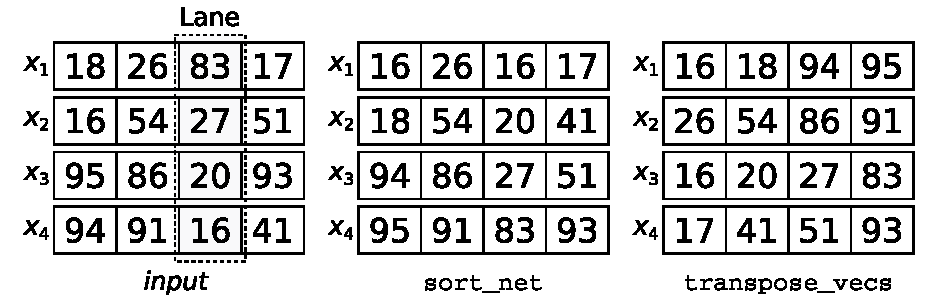
\includegraphics[width=0.99\linewidth]{fig/regs.pdf}}
\caption{Four vectors with four values, the result from a vectorized four-elements sorting network, and the transpose.}
\label{fig:transpose-vecs}
\end{figure}

\subsection{Bitonic Merge Networks}
%
A bitonic sequence starts either increasing or decreasing and contains at most one change of direction. Bitonic merge networks allow the creation of merge networks of different sizes, and they are again implemented in \chipsort in a single generated function, {\tt bitonic\_merge}. Merging two sorted vectors requires first reversing one of them, and the result is stored in two new vectors of the same size containing the first and second halves of the total sorted sequence.

Apart from the use in sorting small sequences and in the multi-way merge tree, bitonic merge networks can also be used to implement a regular merge sort. This technique was investigated in \chipsort only superficially, and while there were no promising results in terms of performance, \chipsort also contains the generated function {\tt bitonic\_merge\_interleaved} to illustrate how metaprogramming can help implementing multiple simultaneous merges with interleaved execution, as done in other projects~\cite{DBLP:journals/pvldb/ChhuganiNLMHCBKD08}.

\subsection{Vectorized Combsort}
%
One of the most peculiar aspects of \chipsort, taken directly from AA-sort~\cite{DBLP:conf/IEEEpact/InoueMKN07,DBLP:journals/pvldb/InoueT15}, is the use of the Combsort algorithm. Combsort is essentially a generalization of Bubble sort in the same way that Shell sort generalizes Insertion sort~\cite{dobosiewicz1980efficient,Lacey:1991:FES:117187.117218,DBLP:books/lib/Knuth98a,DBLP:books/daglib/0023376,INCERPI198737}. The array is swept multiple times, and pairs of values at a given distance from each other are compared and stored in order. The distance is reduced at each pass by a factor of $\frac{4}{3}$. This algorithm lends itself easily to vectorization: performing the comparisons over vectors of size $V$ effectively allows us to run the algorithm over $V$ lists simultaneously.

\chipsort contains two functions that utilize Combsort. The first is {\em chipsort!}, a serial implementation of the algorithm which is vectorized implicitly by the compiler optimizations. {\tt chipsort!} starts with Combsort until the interval size is 1, when it switches to Insertion sort. This is similar to what is often done in practical implementations of Quicksort, as in the Julia standard library, switching to Insertion sort when the array becomes too small. The difference is that Combsort is not a divide-and-conquer approach, and therefore Insertion sort is applied only once through the whole array. Shell sort also terminates naturally applying Insertion sort to a partially sorted array.

The other function is {\tt chipsort\_medium!}, an explicitly vectorized implementation utilizing {\tt SIMD.jl}. This second function also performs a number of other operations before and after using Combsort. It consists of the following steps:
\begin{enumerate}
\item Apply a sorting network on $K$ blocks of $J$ vectors of size $V$.
\item Vectorized Combsort until the interval size is 1.
\item Transpose blocks.
\item Transpose data in-place from $K$ blocks of $J$ vectors into $J$ blocks of $K$ vectors.
\item Vectorized Combsort again.
\item Sort blocks again.
\item Insertion sort.
\end{enumerate}

After the first two steps the result is essentially a matrix where the $K\times J$ columns are the vectors, and each row contains an approximately sorted sequence. The transpose steps reshape each row into a new block. Each row is processed independently at first, and the transpose allows elements from distinct groups to interact. The last step is necessary to ensure the whole array is sorted, not viewed anymore as a matrix with independent rows.

In both implementations switching to Insertion sort presents a better performance than sticking to Combsort until the end. It essentially means using Bubble sort once the interval becomes 1, therefore looking for an alternative seems like a good idea. Insertion sort should fare well because the array is now approximately sorted, and it should not have to move any out-of-order elements very far from where they are found.

Finishing a sorting method with Insertion sort is a common practice, present at least in Musser's Introsort~\cite{musser1997introspective}. The utilization of Insertion sort as a final stage to Combsort has been considered before in the literature~\cite{combwiki,INCERPI198737}, although this method does not seem to enjoy wide adoption. The main contribution of the present work may be to propose again this method in the SIMD context, extending AA-sort~\cite{DBLP:conf/IEEEpact/InoueMKN07,DBLP:journals/pvldb/InoueT15}, bringing experimental evidence of its good performance.

\subsection{In-place matrix transpose}
%
In-place matrix transposition can be attained by moving a number to its destination, then moving the number that was found there, and so on, until a cycle is completed and a new number is selected to be moved~\cite{10.1093/comjnl/2.1.47}. While carrying out this procedure is simple, it is not trivial to find out which are the cycles to tranpose a matrix of any given dimensions, and even finding out the number of cycles turns out to be a difficult problem~\cite[Sec. 1.3.3, Ex. 12]{DBLP:books/lib/Knuth97}.

\chipsort contains the generated function {\tt transpose!} to perform in-place matrix transposition. The cycle seeds are computed at the time of code generation, and at runtime the function only needs to move the data and compute the indices detecting when each cycle finishes. The function is therefore completely generic, supporting any dimensions, but with a very simple runtime code, with the most complex part of the problem being tackled programatically during code generation.

\subsection{Vectorized multi-way merging}
%
Merging multiple arrays simultaneously requires the creation of a {\em merge tree} to keep some intermediate data. Each node in this tree is essentially an iterator traversing the merger of two arrays in the lower level. To employ the vectorized bitonic merge network in this process it is necessary to keep a whole vector at each node of the tree. To produce the next vector of elements one of the two source arrays is selected according to their smallest next element, and a whole vector is pulled from that array. This vector is merged with the intermediate one, and the first half of the resulting sequence can be taken to the next level of the tree, while the second half is kept as the new intermediate data.

Given a set of sorted arrays, once the tree is initialized data is taken from it one vector at a time, producing the final sorted sequence. Each time a new vector is requested the tree is traversed looking for the smallest element between each of the node children, until one of the input arrays is reached. The data from the array is then loaded from memory and merged with the intermediate data, producing new updates moving trought the tree until the root is reached.

The intermediate data from the tree is kept by \chipsort in a contiguous array, treated as a heap. Each node ancestor can be found simply by the Euclidean division of its index by 2. During operation it is assumed this data should fit some level of cache memory, as in the related work~\cite{DBLP:conf/IEEEpact/InoueMKN07,DBLP:journals/pvldb/ChhuganiNLMHCBKD08,DBLP:journals/pvldb/InoueT15}.


\section{Experiments}
\label{sec:experiments}
%
This section reports experiments with the methods offered by the \chipsort library, as well as alternative baseline methods. The term {\it method} can be understood as both the sorting algorithm and their actual implementations in the Julia language. The specific methods tested are:
\begin{itemize}
\item {\tt chipsort!} Combsort finishing with Insertion sort, written as a serial program and vectorized by the compiler.
\item {\tt chipsort\_small!} in-register, based on sorting networks.
\item {\tt chipsort\_medium!} vectorized Combsort, plus additional steps, finishing with Insertion sort.
\item {\tt chipsort\_large} merge-sort with a multi-way merge tree, starting from chunks processed by {\tt chipsort\_medium!}.
\item {\tt insertion\_sort!} Insertion sort taken from the Julia library.
\item {\tt sort!} the Julia standard sort, Quicksort finishing with Insertion sort for small arrays (20 elements).
\end{itemize}

The {\tt !} implies in-place operation. The allocation time for {\tt chipsort\_large} was not discounted in our analyses.

\subsection{Small arrays}
In our first experiment we evaluate the sorting of small arrays, with only 64 32-bit values. The {\tt chipsort\_small} method based on sorting and bitonic merge networks was compared to serial Insertion sort, the Julia sort and {\tt chipsort!}. The small running time makes it challenging to perform proper measurements in this experiment. Our task was therefore to sort 128 sequences of 64 contiguous values in memory, forming a single block of $2^{13}$ uniform random entries. The in-place sorting functions were applied in sequence, in a for-loop. The results are in Table~\ref{tab:bench-small}.

\begin{table}[h]
\tabcolsep22pt
\tbl{Sorting $128 \times 64$ {\tt UInt32} elements.}{
\begin{tabular}{|l|r|}\hline
Method & Median time\\\hline
\chipsort small & 57.206 $\mu$s\\\hline
\chipsort & 133.510 $\mu$s\\\hline
Insertion sort & 194.679 $\mu$s\\\hline
Julia standard & 222.910 $\mu$s\\\hline
\end{tabular}}
\label{tab:bench-small}
\end{table}

The {\tt chipsort\_small} function achieved a significant speed-up of over 3 times compared to Insertion sort or the Julia standard function, and twice over {\tt chipsort!}. Even though the in-register function was clearly faster, this first experiment already demonstrates the potential of {\tt chipsort!}, which presented a speedup of at least 46\% compared to the other alternatives.

\subsection{Medium and large arrays}
In our second experiment we compared many different methods on inputs of exponentially increasing sizes, from $2^6$ up to $2^{20}$. Figure~\ref{fig:bench-time} displays the resulting measurements. Although the curves look too concentrated in this visualization, it is possible to notice that {\tt chipsort!} consistently outperforms the Julia standard library {\tt sort!} by a factor of 80\% to 100\%, or up to twice as fast. We can also observe that Insertion sort soon becomes too inefficient.

\begin{figure}[htb]
\centerline{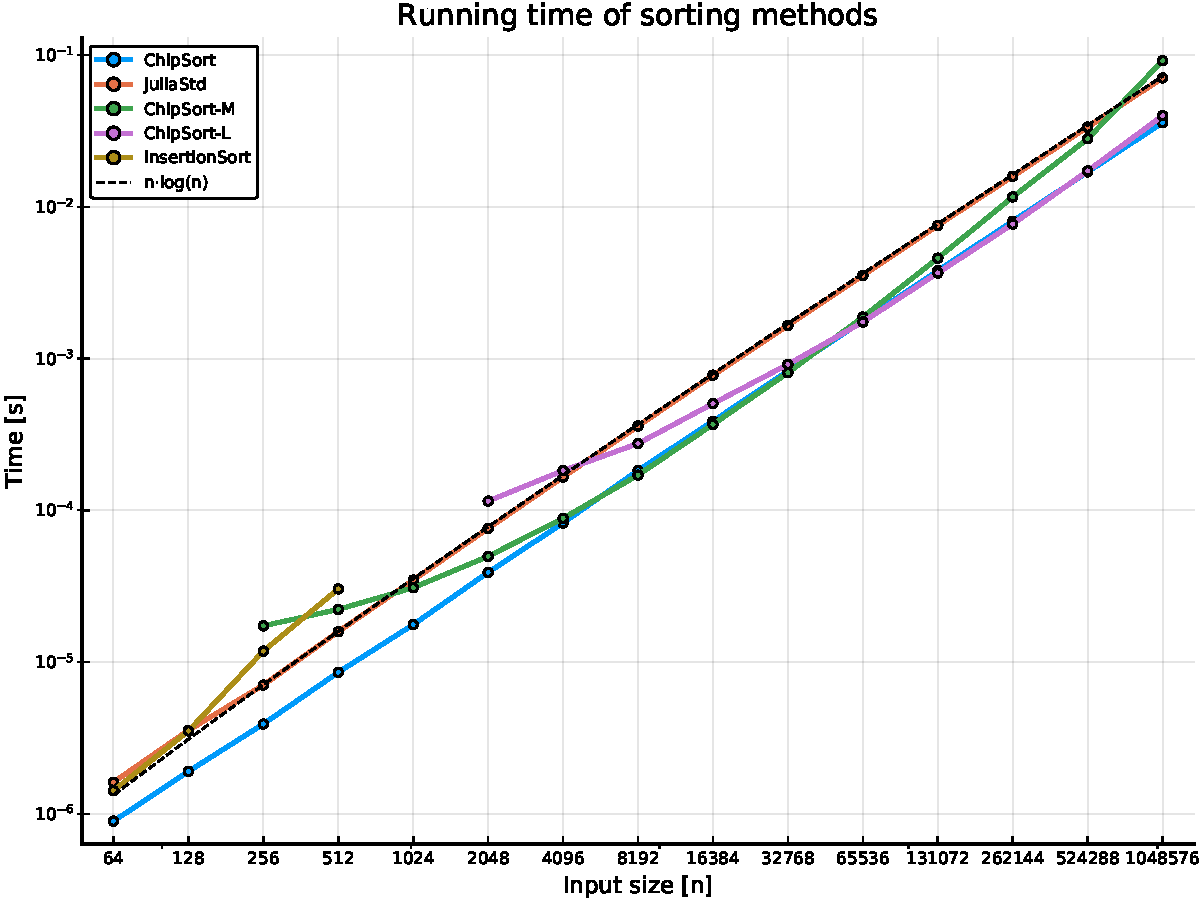
\includegraphics[width=0.99\linewidth]{fig/chipsort-bench-time.pdf}}
\caption{Running time of the different sorting methods studied.}
\label{fig:bench-time}
\end{figure}

Figure~\ref{fig:bench-curves} shows a different visualization from the same data in Figure~\ref{fig:bench-time}, with the times divided by the input size at each point. Here we can see more clearly how {\tt chipsort\_medium} and {\tt chipsort\_large} slightly outperform {\tt chipsort!} in a few cases.

\begin{figure*}[htb]
\centerline{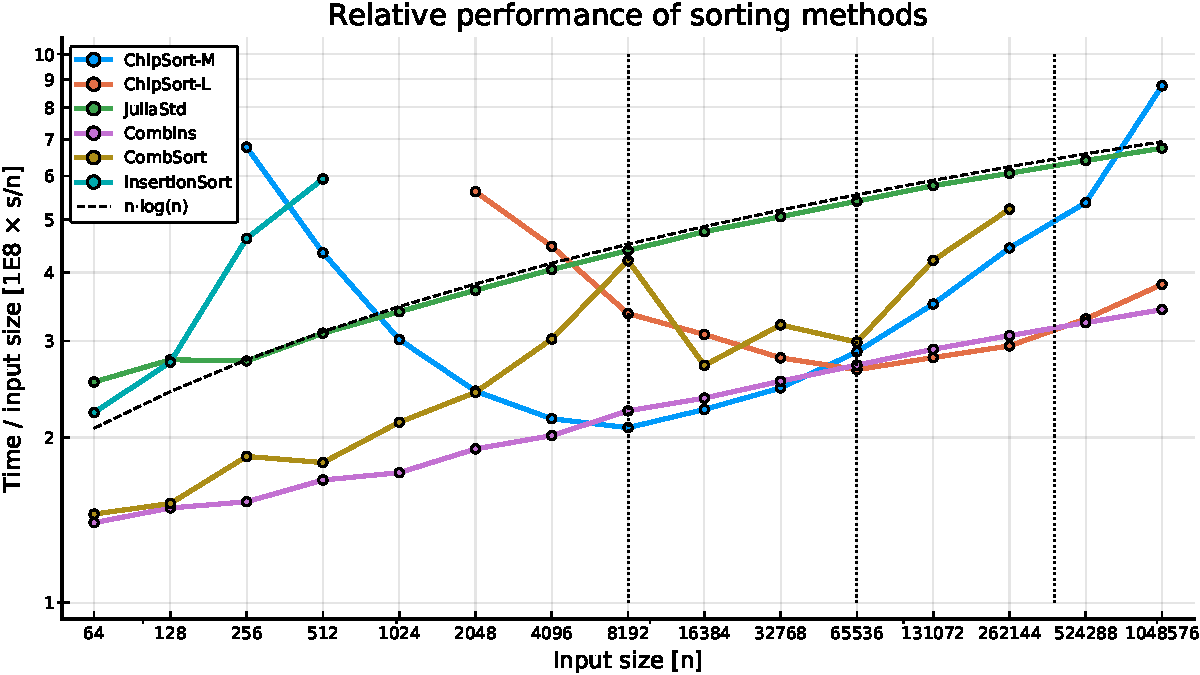
\includegraphics[width=0.75\linewidth]{fig/chipsort-bench-curves.pdf}}
\caption{Curves displaying the relative running time from each studied method. The ordinate represents the median of the measured running times divided by the input size at each test.}
\label{fig:bench-curves}
\end{figure*}

Figure~\ref{fig:bench-cdf} displays the measured times for $2^{13}$ and $2^{18}$ elements. All the tested \chipsort methods surpass the Julia standard library in these cases. In the $2^{13}$ case {\tt chipsort\_medium!} exhibits a slight speedup of 7.3\% over {\tt chipsort!}, and on the $2^{13}$ case it is {\tt chipsort\_large!} with 4.4\%.

\begin{figure}[htb]
\centerline{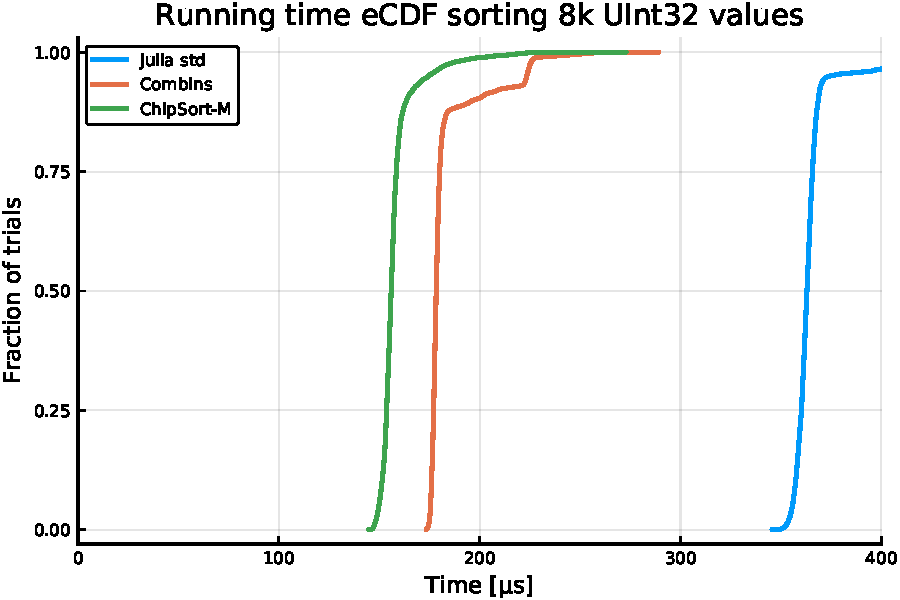
\includegraphics[width=0.99\linewidth]{fig/chipsort-bench-8k.pdf}}
\centerline{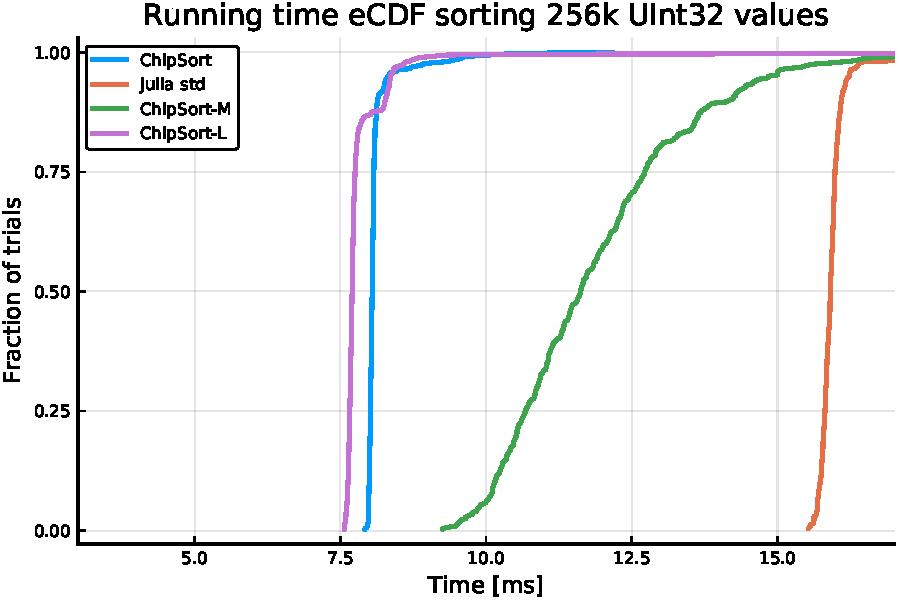
\includegraphics[width=0.99\linewidth]{fig/chipsort-bench-256k.pdf}}
\caption{Empirical CDF from different methods with 8k and 256k {\tt UInt32} values. Results from 10,000 measurements.}
\label{fig:bench-cdf}
\end{figure}

A simple experiment was also carried out with other programming languages in the same machine to provide a richer context. Table~\ref{tab:bench-cxx} diplays statistics collected from Julia, Python and C++ programs. For the case of Python the value obtained when calling the function through PyCall was better than measuring in the native Python shell, therefore the best value was kept. Results obtained for C++ with Julia interopt using Cxx.jl were slightly worse than native, thus discarded. While Numpy was almost as fast as Julia, no reason could be found for the significantly worse performance from the C++ standard libraries. Supposedly there are important optimizations missing.

\begin{table}[h]
\tabcolsep11pt
\tbl{Sorting arrays of 8k and 1M {\tt UInt32} elements in different platforms.}{
\begin{tabular}{|l|r|r|}\hline
Method & 8k & 1M\\\hline
\chipsort & 172.35 $\mu$s & 35.28 ms\\\hline
Julia standard & 345.46 $\mu$s & 68.39 ms\\\hline
Numpy via PyCall & 369.50 $\mu$s & 70.01 ms\\\hline
C++ {\tt std::qsort} & 788.59 $\mu$s & 147.37 ms\\\hline
C++ {\tt std::sort} & 1,207.23 $\mu$s & 224.71 ms\\\hline
\end{tabular}}
\label{tab:bench-cxx}
\end{table}


\section{Conclusion}
\label{sec:conclusion}
%
We have presented \chipsort, a Julia module for SIMD and cache-aware sorting. The main sorting method utilized in \chipsort is Combsort finalized with Insertion sort. This method is based on previous proposals for SIMD sorting~\cite{DBLP:conf/IEEEpact/InoueMKN07,DBLP:journals/pvldb/InoueT15} and other practical sorting methods~\cite{INCERPI198737,musser1997introspective}. This method was implemented as a serial program vectorized by the Julia compiler and LLVM, resulting in a sorting function up to twice as fast as the Julia standard library sort. This performance holds for at least a million 32-bit integers in a conventional computer.

Other techniques available in \chipsort are sorting networks, bitonic merge networks, in-place matrix transpose and a multi-way merge tree. Vectorized in-register sorting, although limited to small powers of 2, proved to deliver speedups of up to 3 times relative to the standard library.

Results were limited for the method dedicated to large arrays, only narrowly surpassing the main \chipsort method in few occasions. Merge-based techniques may be more advantageous when sorting large registers, though.

The main \chipsort method relies heavily on compiler optimizations, while other methods utilize explicit vectorization trough SIMD.jl. \chipsort makes extensive use of metaprogramming, in especial Julia generated functions. This allows functions like sorting networks to be implemented in an abstract and generic way. The networks are represented as data structures, used by a higher-level program to assemble the final network code. This contrasts with other libraries where different networks are implemented straight as final functions. Julia also has the opportunity to performing many optimizations since \chipsort is implemented in pure Julia with abstract methods that can be specialized.

It is a testament to the quality of the Julia compiler infrastructure that the most successful method implemented in \chipsort has no explicit vectorization or intrinsics. It is just a simple, scalar implementation of Combsort that is optimized by the compiler to generate code adapted to different problem settings and to the hardware architecture at run-time. In the cases where explicit vectorization can produce better code, though, Julia still offers a suitable framework that allowed \chipsort to implement sophisticated techniques with concise code. And while this project can illustrate how well Julia implements traditional language features such as parametric types, its metaprogramming features make it stand out from other languages even more.

Some future prospects for \chipsort are to better deal with floating-point comparisons; implement stable sorting of key-register data; explore the limits of in-register processing, especially in modern 512-bit architectures an eventually GPUs; explore how to interact with the compiler in order to produce optimized code for complex tasks such as multi-stage multi-threaded merge sorting of large arrays.




\input{bib.tex}

\end{document}

% Inspired by the International Journal of Computer Applications template

% latexmk -bibtex -pdf paper.tex
